% !TEX root = ../thesis.tex

\chapter{Analytická časť}

In most eukaryotic and prokaryotic organisms the hereditary material is either linear double-stranded DNA 
(deoxyribonucleic acid) molecules or a circular double-stranded DNA molecule. However, some extracellular life forms, 
might use RNA (ribonucleic acid) as the building block for their genome. For instance, viruses have a genome composed of 
either single-stranded DNA, double-stranded DNA or RNA, depending on the type of a virus. Therefore, a genome itself, 
is the complete content of genetic information in an organism, or in other words, all the unique DNA or RNA sequences the organism possesses. 
\section{Nucleotides: the basic subunit of genome}

Both of DNA and RNA  are polymeric molecules, that are composed of linear chains of various combinations of four different subunits, called nucleotides. 
The nucleotide itself is the basic unit of the DNA and RNA molecules, the monomer, which, however, could be found in the cell not only as the bearer of the genetic information, 
but also as a carrier of energy used to power enzymatic reactions. A five-carbon-atom sugar, a phosphate group and a nitrogenous base are three distinct components which, 
combined together, make up the quite complex nucleotide molecule. The combination of sugar and base is called a nucleoside, while the phosphate-sugar-base is termed a nucleotide. 
The nucleotide bases can be either a single-ringed pyrimidine or a double-ringed purine. Dinucleotide, trinucleotide and polynucleotide are the terms corresponding to two, 
three or many nucleotides connected with each other respectively.

\begin{figure}[!ht]
	\centering
	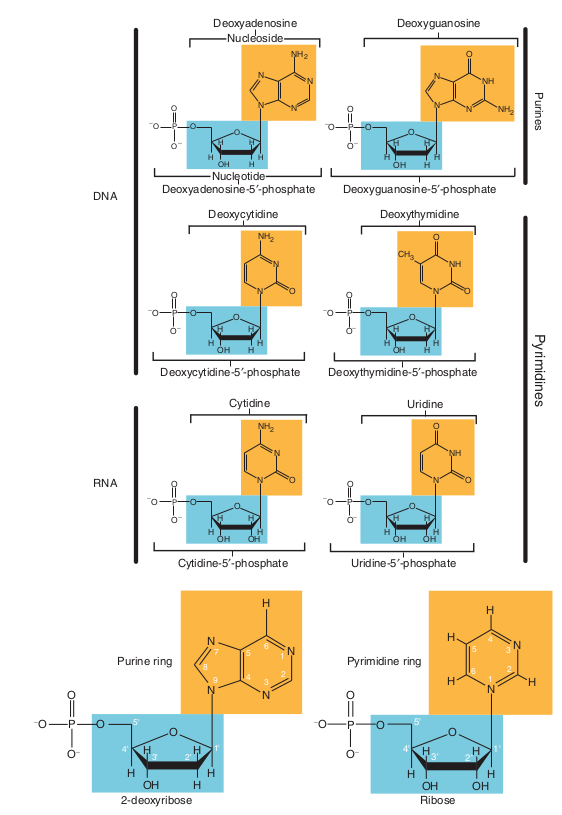
\includegraphics[width=.9\textwidth]{figures/bases}
	\caption{The structures of the pyrimidines and purines found in DNA and RNA. The sugar groups are highlighted in blue and the nitrogenous bases are highlighted in orange. 
	The atoms of the sugar are numbered from 1 to 5. The atoms of the purine ring are numbered from 1 to 9, 
	while those of the pyrimidine ring are numbered from 1 to 6. \label{o:latex_friendly_zone}}
\end{figure}

A nucleotide can be either a purine or pyrimidine. Guanine (G) and adenine (A) are the common purines for both of DNA and RNA; 
the pyrimidine called cytosine (C) is also present in both nucleic acids. However, the pyrimidine uracil (U) is limited only to RNA, 
being replaced with thymine (T) in DNA. There are merely two base-pair combinations that are permissible – A base-paired with T (U) and C base-paired with G. 
It happens due to the geometries of the nucleotide bases and relative positions of atoms which participate in the connection. 
This property makes two sequences of polynucleotides in helix complement. Discrete nucleotides are attached to each other through sugar–phosphate bonds 
that connect the phosphate group on the 5’ carbon of one nucleotide with the hydroxyl group on the 3’ carbon of another nucleotide. 
The base pairing between adenine and thymine (uracil) involves two hydrogen bonds, while between cytosine and guanine involves three hydrogen bonds.
\section{Nucleodic acid spatial stucture}

As the three-dimensional structure of a nucleotide is not completely rigid, it is possible for DNA to have various spatial architectures: 
A-form, B-form, Z-form and the circular one. The position of the base relatively to the five-carbon-atom sugar can be changed by a rotation 
around the N-glycosidic bond and, in this way, significantly affect the three dimensional configuration of the molecule and helix consequently.

\begin{table}[!ht]
	\caption{DNA double helix}\label{t:1}
	\smallskip
	\centering
	
	\begin{tabular}{ |p{3cm}||p{3cm}|p{3cm}|p{3cm}|  }
		\hline
		\multicolumn{4}{|c|}{Features of the different conformations of the DNA double helix} \\
		\hline
		Feature& B-DNA & A-DNA & Z-DNA\\
		\hline
		\hline
		Type of helix & Right-handed & Right-handed & Left-handed\\
		\hline
		Number of base pairs per turn & 10 & 11 & 12\\
		\hline
		Distance between base pairs (nm) & 0.34 & 0.29 & 0.37\\
		\hline
		Distance per complete turn (nm) & 3.4 & 3.2 & 4.5\\
		\hline
		Diameter (nm) & 2.37 & 2.55 & 1.84\\
		\hline
		Major groove & Wide, deep & Narrow, deep & Flat\\
		\hline
		Minor groove & Narrow, shallow & Wide shallow & Narrow, deep\\
		\hline
	\end{tabular}
\end{table}

Moreover, although usually single-stranded, some RNA sequences have the ability to form a double helix. 
However, double helix RNA is rare and has nothing in common with the genome itself, since only the 
single-stranded RNA molecules appear to participate in some genome related processes in the eukaryotic and prokaryotic organisms. 
Since circular DNA may exist in several forms including single-stranded c-DNA, intact double-stranded c-DNA (closed circles with both strands covalently linked), 
nicked ds-c-DNA (only one strand covalently linked) and “concatenated circles” their properties are not described in the attached table.

\section{Eukaryotic genome organization}

In eukaryotic cells nucleic acid is situated in a membrane-bound organelle called the nucleus.
The nuclear genome is split into a set of linear double-helix DNA molecules, each contained in a chromosome. 
No exceptions to this pattern are known: all eukaryotes that have been studied have at least two chromosomes and the DNA molecules are always linear. 
The only variability at this level of organization of eukaryotic genome is coherent with the number of chromosomes. 
Moreover, it appears, that biological features of an organism have no dependence on the number of chromosomes. 

\begin{figure}[!ht]
	\centering
	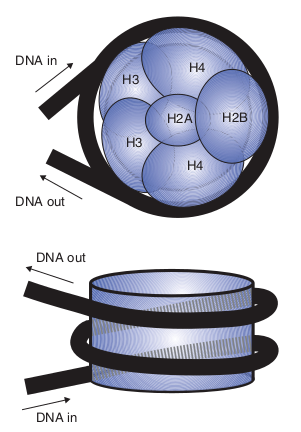
\includegraphics[width=.5\textwidth]{figures/nucleoDetailed}
	\caption{The nucleosome structure. H2A, H2B, H3 and H4 represent different types of histones. \label{o:latex_friendly_zone}}
\end{figure}

Despite the size of a nucleus (5-10 um), an overall length of DNA in the human cell is approximately 2.1m and can be packed inside the cell 
because of the method the nucleic acid is stored. The genetic material in viruses and bacteria consists of strings of DNA or RNA almost devoid of proteins. 
However, in eukaryotes, a substantial quantity of protein is associated with the DNA to form chromatin. At the lowest level, the DNA is organized by 
wrapping DNA strands around he proteins called histones, that contain a large amount of positively charged amino acids arginine and lysine. 
Those amino acids, and histones in general, play the crucial structural role, making it possible to bind the negative charged phosphate groups of the DNA nucleotides.

Averagely, the DNA rolled around the histones consists of 140-150 base pair, dependently on the species. Such a complex of DNA and histones is termed a nucleosome. 
These nucleosomes can be further coiled into increasingly larger coils up until forming chromosomes. However, tight coiling of DNA limits cells ability to access DNA and to process it.
Instead of being constantly coiled, the nucleic acid is usually found in a state called chromatin where some segments of acid are tightly reeled (heterochromatin), 
while other segments are entirely open (euchromatin). Euchromatin DNA is is highly accessible by the molecular complexes used by the cell and therefore is easier to manipulate with. 

The amount and extent of packing are determined by a sell, to control which sections of the genome can be expressed and which cannot. 
It affects cellular function and appears to be the predominant cause of differentiating cells type, while having the same DNA.

\begin{figure}[!ht]
	\centering
	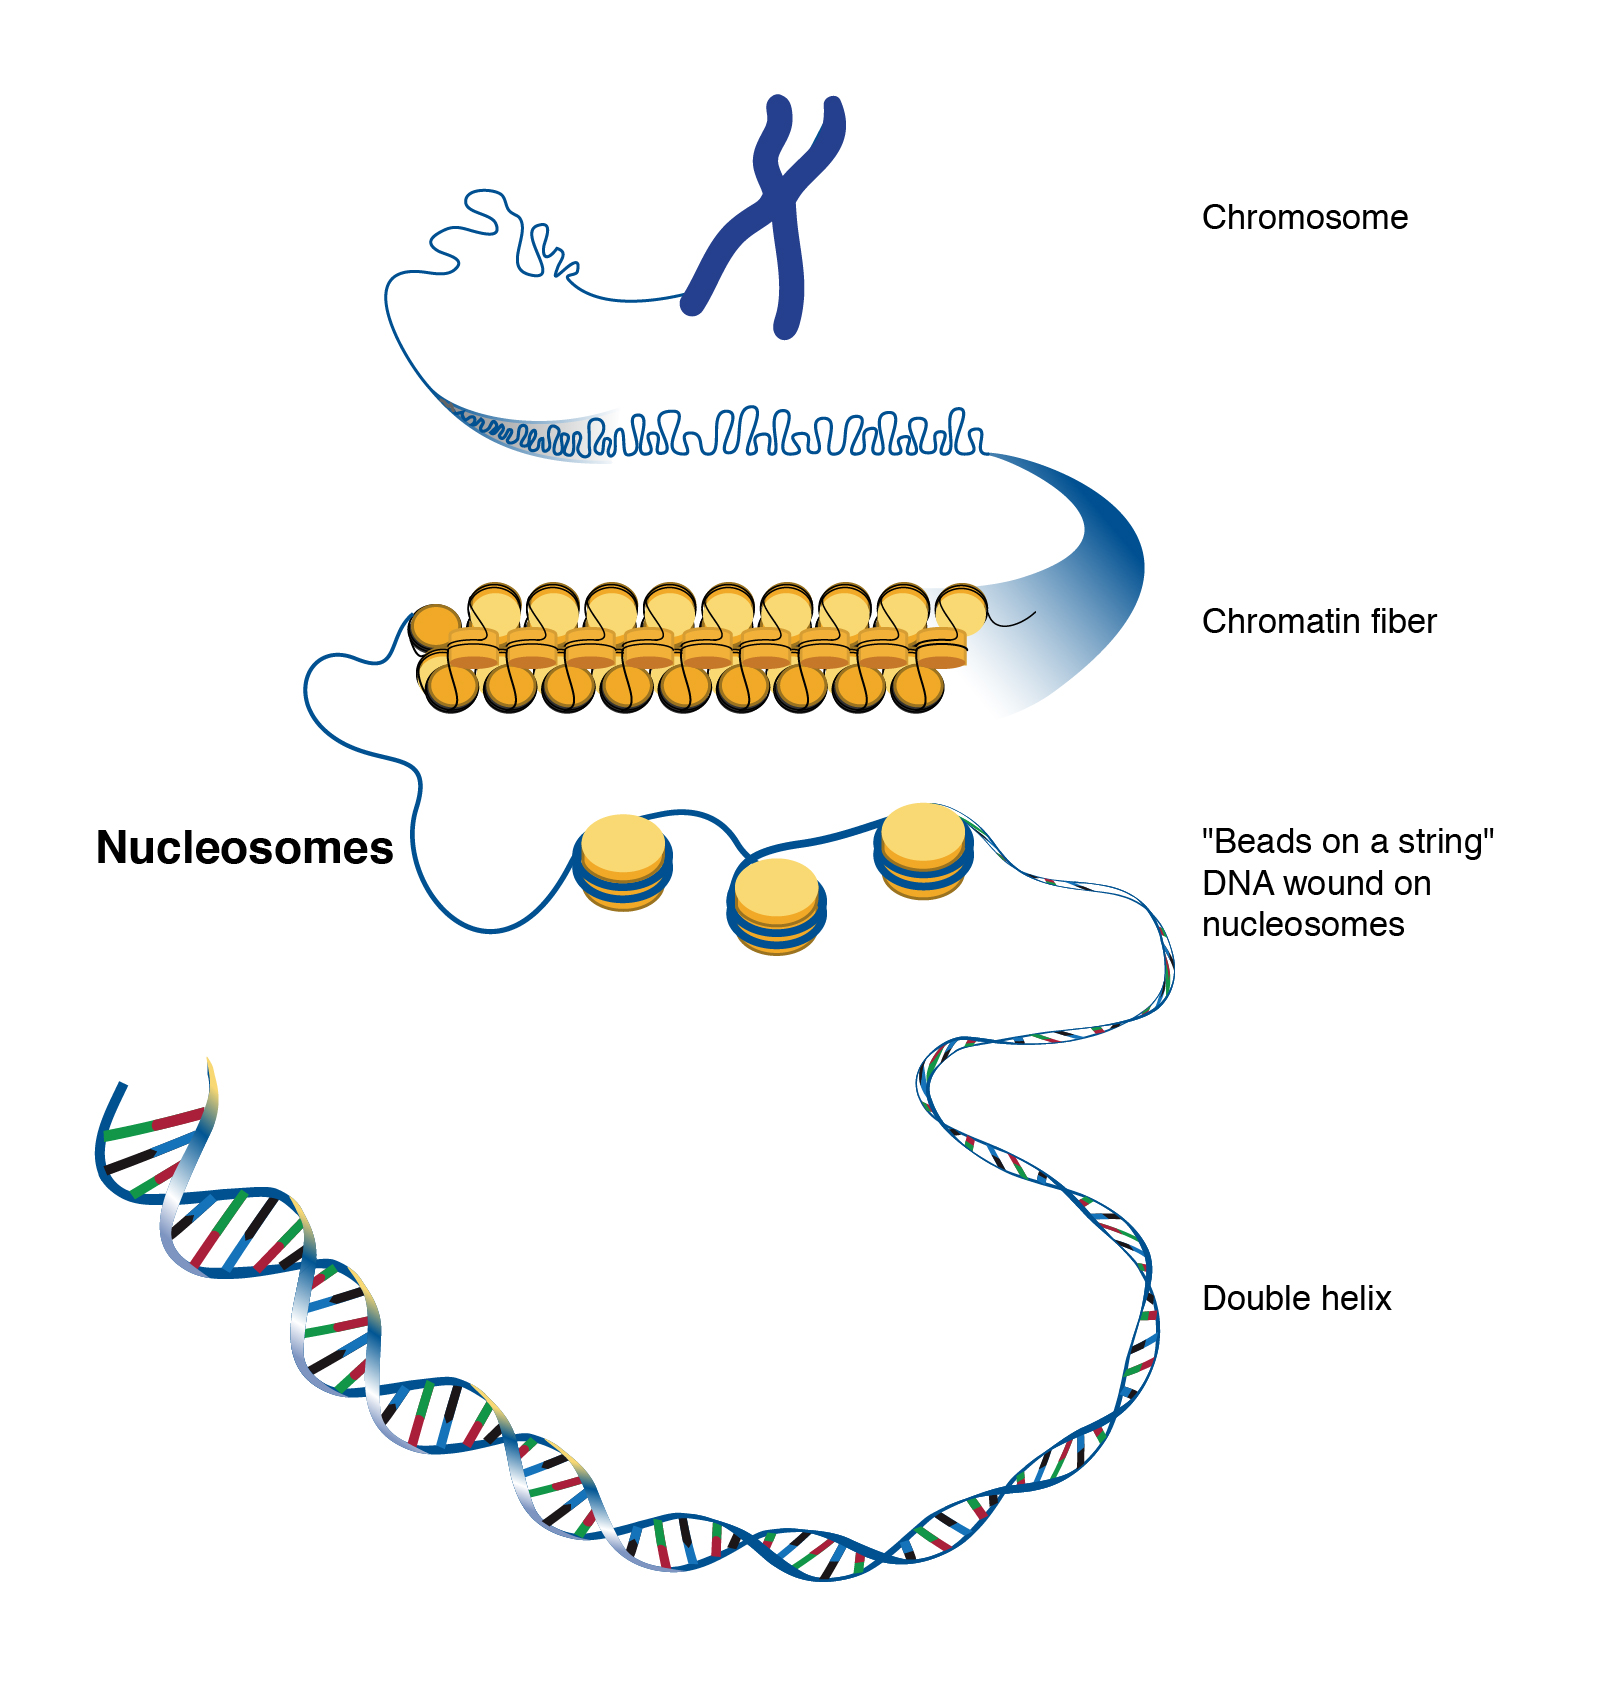
\includegraphics[width=.9\textwidth]{figures/nucleosome1}
	\caption{Ncleosomes as the part of a chromosome.\label{o:latex_friendly_zone}}
\end{figure}

\section{Prokaryotic genome organization}
Prokaryotic genomes are very different from eukaryotic ones, in particular with regard to the physical organization of the genome within the cell.
Although the word “chromosome” is used to describe the DNA–protein structures present in prokaryotic cells, this is a misnomer as this structure has few
similarities with a eukaryotic chromosome. 
The traditional view has been that in a typical prokaryote the genome is contained in a single, circular DNA molecule, 
localized within the nucleoid — the lightly staining region of the otherwise featureless prokaryotic cell. This is certainly true for E. coli and many of the other 
commonly studied bacteria.

Most of what we know about the organization of DNA in the nucleoid comes from studies of E. coli. The first feature to be recognized was that the circular
E. coli genome is supercoiled. Supercoiling occurs when additional turns are introduced into the DNA double helix (positive supercoiling) or if turns are
removed (negative supercoiling). With a linear molecule, the torsional stress introduced by over- or underwinding is immediately released by rotation of
the ends of the DNA molecule, but a circular molecule, having no ends, cannot reduce the strain in this way. Instead the circular molecule responds by
winding around itself to form a more compact structure. Supercoiling is therefore an ideal way to package a circular molecule into a small space. 
Evidence that supercoiling is involved in packaging the circular E.coli genome was first obtained in the 1970s from examination of isolated nucleoids, 
and subsequently confirmed as a feature of DNA in living cells in 1981. In E. coli, the supercoiling is thought to be generated and controlled by two enzymes, 
DNA gyrase and DNA topoisomerase I.

The E. coli genome, as described above, is a single, circular DNA molecule. This is also the case with the vast majority of bacterial and archaeal chromosomes 
that have been studied, but an increasing number of linear versions are being found. The first of these, for Borrelia burgdorferi, the organism that causes 
Lyme disease, was described in 1989, and during the following years similar discoveries were made for Streptomyces coelicolor and Agrobacterium tumefaciens. 
Linear molecules have free ends, which must be distinguishable from DNA breaks, so these chromosomes require terminal structures equivalent to the telomeres 
of eukaryotic chromosomes. In Borrelia and Agrobacterium, the real chromosome ends are distinguishable because a covalent linkage is formed 
between the 5` and 3` ends of the polynucleotides in the DNA double helix, and in Streptomyces the ends appear to be marked by special binding proteins.

\section{Genes: location and general structure}
Gene is a sequence of nucleotides in DNA or RNA that encodes the synthesis of a gene product, either RNA or protein that have distinctive features. At present we 
do not fully understand the nature of all of these specific features, and sequence inspection is therefore not a foolproof way of locating genes. 
Genes that code for proteins comprise open reading frames (ORFs) consisting of a series of codons that specify the amino acid sequence of the protein
that the gene codes for. The ORF begins with an initiation codon—usually (but not always) ATG — and ends with a termination codon: TAA, TAG, or TGA. 
Searching a DNA sequence for ORFs that begin with an ATG and end with a termination triplet is therefore one way of looking for genes. The analysis is 
complicated by the fact that each DNA sequence has six reading frames, three in one direction and three in the reverse direction on the complementary strand.

\begin{figure}[!ht]
	\centering
	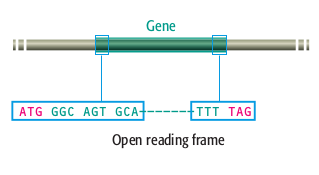
\includegraphics[width=.9\textwidth]{figures/ORF1.png}
	\caption{The
	first four and last two codons of the gene
	are shown. The first four codons specify
	methionine/initiation–glycine–serine–alanine,
	and the last two specify
	phenylalanine–termination.\label{o:latex_friendly_zone}}
\end{figure}


The key to the success of ORF scanning is the frequency with which termination codons appear in the DNA sequence. If the DNA has a random sequence
and a GC content of 50\% then each of the three termination codons — TAA, TAG, and TGA — will appear, on average, once every 64 bp. If the GC content 
is greater than 50\% then the termination codons, being AT – rich, will occur less frequently, but one will still be expected every 100–200 bp. This
means that random DNA should not show many ORFs longer than 50 codons in length, especially if the presence of a starting ATG triplet is used as part of
the definition of an ORF. Most genes, on the other hand, are longer than 50 codons: the average lengths are 317 codons for Escherichia coli, 483 codons
for Saccharomyces cerevisiae, and approximately 450 codons for humans. ORF scanning, in its simplest form, therefore takes a figure of, say, 100 codons
as the shortest length of a putative gene and records positive hits for all ORFs longer than this.


With bacterial genomes, simple ORF scanning is an effective way of locating most of the genes in a DNA sequence. shows a segment of the E. The real genes
in the sequence cannot be mistaken because they are much longer than 50 codons in length. With bacteria the analysis is further simplified by the fact
that the genes are very closely spaced and hence there is relatively little intergenic DNA in the genome (only 11\% for E. coli). If we assume that the 
real genes do not overlap, which is true for most bacterial genes, then it is only in the intergenic regions that there is a possibility of mistaking a short, 
spurious ORF for a real gene. So if the intergenic component of a genome is small, then there is a reduced chance of making mistakes in 
interpreting the results of a simple ORF scan. 

\begin{figure}[!ht]
	\centering
	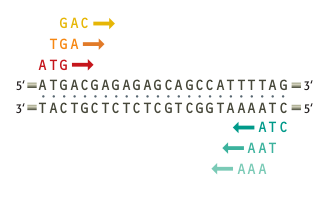
\includegraphics[width=.9\textwidth]{figures/ORF2.png}
	\caption{Both
	strands are read in the 5¢Æ3¢direction. Each
	strand has three reading frames, depending
	on which nucleotide is chosen as the
	starting position.\label{o:latex_friendly_zone}}
\end{figure}

Although ORF scans work well for bacterial genomes, they are less effective for locating genes in DNA sequences from higher eukaryotes. This is partly
because there is substantially more space between the real genes in a eukaryotic genome (for example, approximately 62\% of the human genome is intergenic), 
increasing the chances of finding spurious ORFs. But the main problem with the human genome and the genomes of higher eukaryotes in general is that their 
genes are often split by introns, and so do not appear as continuous ORFs in the DNA sequence. Many exons are shorter than 100 codons, some consisting of 
fewer than 50 codons, and continuing the reading frame into an intron usually leads to a termination sequence that appears to close the ORF. In other words, 
the genes of a higher eukaryote do not appear in the genome sequence as long ORFs, and simple ORF scanning cannot locate them.

Solving the problem posed by introns is the main challenge for bioinformaticists writing new software programs for ORF location. A good example of such software
is Glimmer. It uses machine learning for predicting the gene locations. Three modifications to the basic procedure for ORF scanning are usually adopted:

\begin{itemize}
	\item Codon bias is taken into account. “Codon bias” refers to the fact that not all codons are used equally frequently in the genes of a particular organism. 
	For example, leucine is specified by six codons in the genetic code (TTA, TTG, CTT, CTC, CTA, and CTG), but in human genes leucine is most frequently coded by 
	CTG and is only rarely specified by TTA or CTA. Similarly, of the four valine codons, human genes use GTG four times more frequently than GTA. The biological 
	reason for codon bias is not understood, but all organisms have a bias, which is different in different species. Real exons are expected to display the codon 
	bias whereas chance series of triplets do not. The codon bias of the organism being studied is therefore written into the ORF-scanning software.

	\item Exon–intron boundaries can be searched for as these have distinctive sequence features, although unfortunately the distinctiveness of these
	sequences is not so great as to make their location a trivial task. The sequence of the upstream exon–intron boundary is usually described as:
	5'–AGØGTAAGT–3' the arrow indicating the precise boundary point. However, only the “GT” immediately after the arrow is invariable: elsewhere in the sequence,
	nucleotides other than the ones shown are quite often found. In other words, the sequence is a consensus, by which we mean that the sequence shows the
	most frequent nucleotide at each position in all of the upstream exon–intron boundaries that are known, but that in any particular boundary sequence
	one or more of these positions might have a different nucleotide. The downstream intron–exon boundary is even less well defined: 5'–PyPyPyPyPyPyNCAGØ–3'
	where “Py” means one of the pyrimidine nucleotides (T or C) and “N” is any nucleotide. Simply searching for these consensus sequences will not
	locate more than a few exon–intron boundaries because most have sequences other than the ones shown. Writing software that takes account of the 
	known variables has proven difficult, and at present locating exon–intron boundaries by sequence analysis is a hit-and-miss affair.

	\item Upstream regulatory sequences can be used to locate the regions where genes begin. This is because these regulatory sequences, like exon–intron
	boundaries, have distinctive sequence features that they possess in order to carry out their role as recognition signals for the DNA-binding proteins
	involved in gene expression. Unfortunately, as with exon–intron boundaries, the regulatory sequences are variable, more so in eukaryotes than in prokaryotes, 
	and in eukaryotes not all genes have the same collection of regulatory sequences. Using these to locate genes is therefore problematic.
\end{itemize}

These three extensions of simple ORF scanning, despite their limitations, are generally applicable to the genomes of all higher eukaryotes. Additional
strategies are also possible with individual organisms, based on the special features of their genomes. For example, vertebrate genomes contain CpG
islands upstream of many genes, these being sequences of approximately 1kb in which the GC content is greater than the average for the genome as a
whole. Some 40\%–50\% of human genes are associated with an upstream CpG island. These sequences are distinctive and when one is located in vertebrate
DNA, a strong assumption can be made that a gene begins in the region immediately downstream.

ORF scanning is appropriate for protein-coding genes, but genes for functional RNAs such as rRNA and tRNA do not comprise open reading frames and hence 
will not be located by the methods described above. Functional RNA molecules do, however, have their own distinctive features, which can be used to aid 
their discovery in a genome sequence. The most important of these features is the ability to fold into a secondary structure, such as the cloverleaf 
adopted by tRNA molecules. These secondary structures are held together by base pairing not between two separate polynucleotides, as in the DNA double helix, 
but between different parts of the same polynucleotide—what we call intramolecular base pairing. In order for intramolecular base pairs to form, the
nucleotide sequences in the two parts of the molecule must be complementary, and to produce a complex structure such as the cloverleaf, the components of these 
pairs of complementary sequences must be arranged in a characteristic order within the RNA sequence. These features provide a wealth of information that 
can be used to locate tRNA genes in a genome sequence, and programs designed for this specific purpose are usually very successful.

As well as tRNAs, rRNAs and some of the small functional RNAs also adopt secondary structures that have sufficient complexity to enable their genes 
to be identified without too much difficulty. Other functional RNA genes are less easy to locate because the RNAs take up structures that involve 
relatively little base pairing or the base pairing is not in a regular pattern. Three approaches are being used for location of the genes for these RNAs:

\begin{figure}[!ht]
	\centering
	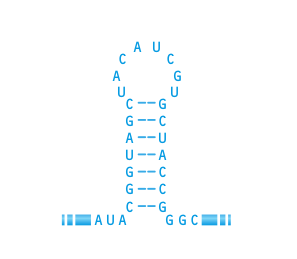
\includegraphics[width=.9\textwidth]{figures/rna.png}
	\caption{A typical RNA stem-loop
	structure.\label{o:latex_friendly_zone}}
\end{figure}

Most of the various software programs available for gene location by ORF scanning can identify up to 95\% of the coding regions in a eukaryotic
genome, but even the best ones tend to make frequent mistakes in their positioning of the exon–intron boundaries, and identification of spurious ORFs as
real genes is still a major problem. These limitations can be offset to a certain extent by the use of a homology search to test whether a series of triplets is a
real exon or a chance sequence. In this analysis the DNA databases are searched to determine if the test sequence is identical or similar to any genes
that have already been sequenced. Obviously if the test sequence is part of a gene that has already been sequenced by someone else then an identical
match will be found, but this is not the point of a homology search. Instead the intention is to determine if an entirely new sequence is similar to any
known genes because, if it is, then there is a chance that the test and match sequences are homologous, meaning that they represent genes that are evolutionarily related. 


\begin{itemize}
	\item Although some functional RNAs do not adopt complex secondary structures, most contain one or more stem-loops (or hairpins), which result
	from the simplest type of intramolecular base pairing. Programs that scan DNA sequences for such structures therefore identify regions where 
	functional RNA genes might be present. These programs incorporate thermodynamic rules that enable the stability of a stem-loop to be estimated, 
	taking into account features such as the size of the loop, the number of base pairs in the stem, and the proportion of G–C base pairs 
	(these being more stable than A–T pairs as they are held together by three rather than two hydrogen bonds). A putative stemloop structure 
	with an estimated stability above a chosen limit is considered a possible indicator of the presence of a functional RNA gene.

	\item As with protein-coding genes, a search can be made for regulatory sequences associated with genes for functional RNAs. These regulatory
	sequences are different to those for protein-coding genes, and may be present within a functional RNA gene as well as upstream of it.

	\item In compact genomes, attention is directed toward regions that remain after a comprehensive search for protein-coding genes. Often these
	“empty spaces” are not empty at all and a careful examination will reveal the presence of one or more functional RNA genes.
\end{itemize}

The main use of homology searching is to assign functions to newly discovered genes, and we will therefore return to it when we deal
with this aspect of genome analysis later in the chapter. The technique is also central to gene location because it enables tentative exon
sequences located by ORF scanning to be tested for functionality. If the tentative exon sequence gives one or more positive matches after a homology
search then it is probably a real exon, but if it gives no match then its authenticity must remain in doubt until it is assessed by one or other of 
the experiment-based gene location techniques.

A more precise version of homology searching is possible when genome sequences are available for two or more related species. Related species have
genomes that share similarities inherited from their common ancestor, overlaid with species-specific differences that have arisen since the species began
to evolve independently. Because of natural selection, the sequence similarities between related genomes are greatest within the genes and lowest in the 
intergenic regions. Therefore, when related genomes are compared, homologous genes are easily identified because they have high sequence similarity, 
and any ORF that does not have a clear homolog in the second genome can be discounted as almost certainly being a chance sequence and not a genuine gene. 
This type of analysis — called comparative genomics — is proving very valuable for locating genes in the Saccharomyces cerevisiae genome, as complete or partial
sequences are now available not only for this yeast but also for 16 other members of the Hemiascomycetes, including Saccharomyces paradoxus,
Saccharomyces mikatae, and Saccharomyces bayanus, the species most closely related to S. cerevisiae. Comparisons between these genomes have
confirmed the authenticity of a number of S. cerevisiae ORFs, and also enabled almost 500 putative ORFs to be removed from the S. cerevisiae catalog on the 
grounds that they have no equivalents in the related genomes. The analysis is made even more powerful by the synteny—conservation of gene
order—displayed by the genomes of these related yeasts. Although each genome has undergone its own species-specific rearrangements there are still
substantial regions where the gene order in the S. cerevisiae genome is the same as in one or more of the related genomes. This makes it very easy to
identify homologous genes but, more importantly, enables a spurious ORF, especially a short one, to be discarded with great confidence, because its
expected location in a related genome can be searched in detail to ensure that no equivalent is present.